\chapter{Mathematical Modelling}\label{ch:mathmodel}

\section{Pump Curves}\label{sec:pumpcurves}
\todo[color=04mathematicalModelling]{static modeling and control + dynamic modeling and control}
\subsubsection{QH-Curve}

A QH-curve or pump curve defines the head as a function of the flow. The flow is the rate of the fluid going through the 
pump. It is generally stated in cubic meter per hour $[m^{3}/h]$. Figure \ref{fig:pump_head_curve} represents a typical pump head curve.

\begin{figure}[h]
	\centering
	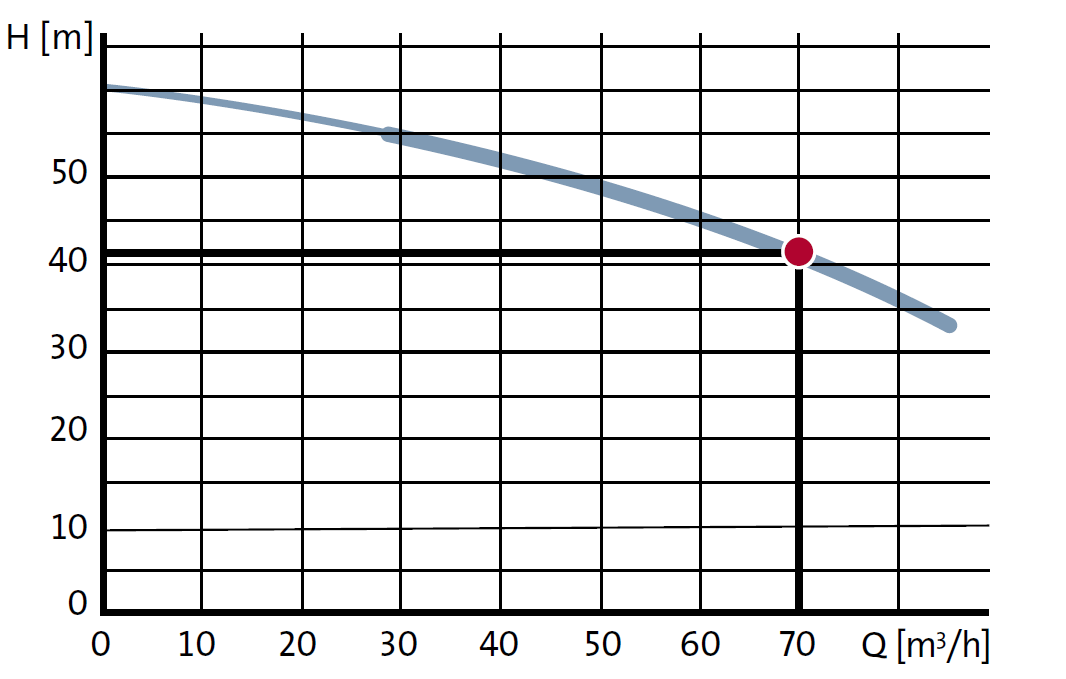
\includegraphics[width = 0.8\linewidth]{figures/pump_head_curve.PNG}
	\caption{Pump Head Curve}
	\label{fig:pump_head_curve}
\end{figure}

\newpage
\subsubsection{System Head Curve}
A system head curve is a graphical representation of the pump head that is required to move fluid through a piping system at various flow rates.
The system curve helps quantify the resistance in a system due to friction and elevation change over the range of flows. 


We used the data gathered through experiments to develop a model that would fit all our data, within a certain degree of error, 
and that we would be able to further test.

We decided to use black-box modeling with polynomial fitting. We based our decision on other research that has been done on the same
setup as ours, and also on the affinity laws.
\todo[color=04mathematicalModelling]{quote zhenyu paper}

Curve Fitting Tool \cite{cftool} \textit{cftool} was used in order to find a suitable mathematical formula for accurately describing the 
system, while also trying to represent it in the easiest manner possible. 
\subsubsection{Single Variable Speed Pump Model}
Equation \ref{eq:pump_model} determines the head and the power, given the flow. 
Although the formula does not directly relate to the pump speed, it indirectly relates to it, due to the fact that only one possible 
pump speed $\omega$ exists for a given flow.
\todo[color=04mathematicalModelling]{maybe say that one pump speed corresponds to a certain flow if everything else is constant}
\todo[color=04mathematicalModelling]{quote zhenyu paper again}

\begin{equation}
	\begin{aligned}
	H = \bar{a_{0}} \cdot Q^2 + \bar{a_{1}} \cdot Q + \bar{a_{2}} \\
	P = \bar{b_{0}} \cdot Q^3 + \bar{b_{1}} \cdot Q^2 + \bar{b_{2}} \cdot Q + \bar{b_{3}}
	\end{aligned}
	\label{eq:pump_model}
\end{equation}

The coefficients are determined by the pump characteristics and can be experimentally identified.

Taking variable speed into account, the equations \ref{eq:pump_model} will depend on the motor speed. 
The pump Affinity Laws state:

\begin{align}
	\left(\frac{\omega_1}{\omega_2}\right)^1 = \frac{Q_1}{Q_2} && 
	\left(\frac{\omega_1}{\omega_2}\right)^2 = \frac{H_1}{H_2} &&
	\left(\frac{\omega_1}{\omega_2}\right)^3 = \frac{P_1}{P_2}	
\end{align}

\newpage
Assuming the pump model parameters ($\bar{a_{0}}$, $\bar{a_{1}}$, $\bar{a_{2}}$) and ($\bar{b_{0}}$, $\bar{b_{1}}$, $\bar{b_{2}}$, $\bar{b_{3}}$) 
described in equation \ref{eq:pump_model} are obtained at a certain speed $\bar{\omega_{0}}$, 
this results in the following equation describing the pump at any speed $\omega$.
\begin{equation}
	\begin{aligned}
	H(\omega) = a_0 \cdot \omega^2 + a_1 \cdot \omega \cdot Q(\omega) + a_2 \cdot Q(\omega)^2 \\
	P(\omega) = b_0 \cdot \omega^3 + b_1 \cdot \omega^2 \cdot Q(\omega) + b_2 \cdot \omega \cdot Q(\omega)^2 + b_3 \cdot Q(\omega)^3
	\end{aligned}
\end{equation}

The coefficients can be determined as follows:

\begin{align*}
	a_0 = \frac{\bar{a_0}}{\bar{\omega_0^2}} && a_1 = \frac{\bar{a_1}}{\bar{\omega_0}} && a_2 = \bar{a_2} \\
	b_0 = \frac{\bar{b_0}}{\bar{\omega_0^3}} && b_1 = \frac{\bar{b_1}}{\bar{\omega_0^2}} && b_2 = \frac{\bar{b_2}}{\omega_0} && b_3 = \bar{b_3}
\end{align*}

Results of the model can be seen in figure and figure.
\todo[color = 04mathematicalModelling]{add figures}
\subsubsection{Multi Variable Speed Pump Model at Same Speed}
For a certain number of pumps P in parallel, with the requirement that they all run at the same speed $\omega$, the pump model is
described by the following equations:

\begin{equation}
	\begin{aligned}
	H_s(\omega) = a_0^s \cdot \omega^2 + a_1^s \cdot \omega \cdot Q_s(\omega) + a_2^s \cdot Q_s(\omega)^2 \\
	P_s(\omega) = b_0^s \cdot \omega^3 + b_1^s \cdot \omega^2 \cdot Q_s(\omega) + b_2^s \cdot \omega \cdot Q_s(\omega)^2 + b_3^s \cdot Q_s(\omega)^3
	\end{aligned}
\end{equation}

The formulas are identical, however the coefficients differ. They can be determined as follows:
\begin{align*}
	a_0^s = a_0 && a_1^s = \frac{a_1}{P} && a_2^s = \frac{a_2}{P^2} \\
	b_0^s = b_0 && b_1^s = \frac{b_1}{P} && b_2^s = \frac{b_2}{P^2} && b_3^s = \frac{b_3}{P^3}
\end{align*}
\todo[color=04mathematicalModelling]{very much from zhenyu's papers, should be able to understand and explain, otherwise, will take out and rewrite}

\newpage
The model has an adjusted coefficient of determination  $\bar{R^2}$ = 1. Such a high coefficient of determination, was achieved due to
heavy filtering of the data gathered. In addition, no, or minor disturbances were present during the gathering of the data.
\todo[color=04mathematicalModelling]{from supervisor meeting} 

The model could be more expanded, reaching a higher order polynomial. However, we have decided the model represents the pump behavior 
accurately enough. Further expansion would result in a higher degree polynomial but not much gain in terms of accuracy.

Using the model shown in Equation \ref{eq:simulated_power} we were able to replicate our data with a small error percentage. The results
are shown in the figures below.
\todo[color=04mathematicalModelling]{not sure if we need this or not so i didn't put any photos}
\newpage
With the data gathered through the experiments (Section \ref{sec:experiment}\todo[color=04mathematicalModelling]{not linked yet}),

\todo[color=04mathematicalModelling]{re-write this section, all math used here doesn't apply to real life. But use the knowledge we 
gained here instead of deleting everything}
We decided to use black-box modelling with polynomial fitting.
For this we used the Curve Fitting Tool \cite{cftool} \textit{cftool} 
\todo[color=04mathematicalModelling]{make this look like a command} in MATLAB.
Looking at the data we decided to use polynomial fitting with a second degree polynomial
as can be seen in equation \ref{eq:polynom}.

\begin{equation}
	 P(Q) = p_1 \cdot Q^2 + p_2 \cdot Q + p_3
	 \label{eq:polynom}
\end{equation}

After repeating this process over different datasets with different pump speeds,
we noticed that the coefficients $p_1$ and $p_2$ barely change.
\todo[color=04mathematicalModelling]{they do, shit isn't even properly linear...}

The standard deviation for the $p_1$ and $p_2$ coefficients were calculated with the equation \todo[color=04mathematicalModelling]{add 
reference to eq}

\begin{equation}
	\sigma_{\mean{p_{1,2}}} = \dfrac{1}{n}\sum |p_{1,2}-\mean{p_{1,2}}|
	\label{eq:avedev}
\end{equation}

The results obviously vary between runs. For the run used to create the model the $\sigma_{\mean{p_{1,2}}}$ are:
\begin{equation}
	\sigma_{\mean{p_1}} \simeq 0.003854$$
	
	$$\sigma_{\mean{p_2}} \simeq 0.042299
\end{equation}

The $p_3$ coefficient however changes significantly, through different pump speeds.
With a standard deviation $\sigma_{\mean{p_3}} \simeq 3.378111$ it was impossible to use only one simple polynomial as described in 
\ref{eq:polynom} to describe all pump characteristics at all speeds.

We were able to identify a second order polynomial describing the change in $p_3$ according to the pump speed $\omega$.
\begin{equation}
	 p_3 = a \cdot \omega^2 + b \cdot \omega + c
	 \label{eq:p3olynom}
\end{equation}

Combining \ref{eq:polynom} and \ref{eq:p3olynom}, we get:

\begin{equation}
	P(Q) = p_1 \cdot Q^2 + p_2 \cdot Q + a \cdot \omega^2 + b \cdot \omega + c 
\end{equation}
\todo[color=04mathematicalModelling]{at least something that isn't completely wrong, but incomplete. Not sure if we should start 
remodelling with power anyways}
